\documentclass[11pt]{article}
%%\documentclass{book}
\usepackage{geometry}            % See geometry.pdf to learn the layout options. There are lots.
\usepackage{xspace}
\geometry{letterpaper}           % ... or a4paper or a5paper or ... 
%\geometry{landscape}            % Activate for for rotated page geometry
%\usepackage[parfill]{parskip}   % To begin paragraphs with an empty line rather than an indent
\usepackage{graphicx}
\usepackage{amssymb}
\usepackage{alltt}
%\usepackage{epstopdf}
%\DeclareGraphicsRule{.tif}{png}{.png}{`convert #1 `dirname #1`/`basename #1 .tif`.png}
\usepackage[T1]{fontenc}   % so _, <, and > print correctly in text.
\usepackage[strings]{underscore}    % to use "_" in text

\usepackage{hyperref}

%---------------------------------------------------------------------------------

\newcommand{\srthree}{\texttt{SYNRAD3D}\xspace}
\newcommand\ttcmd{\begingroup\catcode`\_=11 \catcode`\%=11 \dottcmd}
\newcommand\dottcmd[1]{\texttt{#1}\endgroup}
\newcommand{\Begineq}{\begin{equation}}
\newcommand{\Endeq}{\end{equation}}
\newcommand{\fig}[1]{Figure~\ref{#1}}
\newcommand{\vn}{\ttcmd}           
\newcommand{\Th}{$^{th}$\xspace}
\newcommand{\Newline}{\hfil \\}

\newlength{\dPar}
\newlength{\ExBeg}
\newlength{\ExEnd}
\setlength{\dPar}{1.5ex}
\setlength{\ExBeg}{-\dPar}
\addtolength{\ExBeg}{-0.5ex}
\setlength{\ExEnd}{-\dPar}
\addtolength{\ExEnd}{-0.0ex}

\newenvironment{example}
  {\vspace{\ExBeg} \begin{alltt}}
  {\end{alltt} \vspace{\ExEnd}}

%---------------------------------------------------------------------------------

\setlength{\textwidth}{6.25in}
\setlength{\hoffset}{0.0in}
\setlength{\oddsidemargin}{0.25in}
\setlength{\evensidemargin}{0.0in}
\setlength{\textheight}{8.5in}
\setlength{\topmargin}{0in}

\setlength{\parskip}{\dPar}
\setlength{\parindent}{0ex}

%---------------------------------------------------------------------------------

\title{ \srthree information}
\author{G. Dugan, D. Sagan}
\date{April 25, 2010}

\begin{document}
\maketitle

%------------------------------------------------------------------
\section{Introduction} 

\srthree is a program which simulates
the production and scattering of synchrotron radiation generated by an
electron beam in a high energy machine. The program was written by David
Sagan of Cornell University.

The principal motivation for this simulation is to estimate the
distribution of photon absorption sites around the vacuum chamber as a
function of longitudinal position in the machine. This information is
then input to simulation programs such as \vn{POSINST} and
\vn{ECLOUD}, which simulate photoelectron production in various
magnetic environments, which seeds the formation of the electron
cloud.

\srthree is not to be confused with an older program called
\vn{SYNRAD}. The \vn{SYNRAD} program is used for calculating
wall heating from the primary beam.  \vn{SYNRAD} only tracks
photons in the horizontal plane and does not simulate scattering of
the photons from the wall. The advantage of \vn{SYNRAD} is that it
is fast and directly gives wall heating numbers. The advantage of
\srthree is that it tracks photons in three dimensions and it does
simulate scattering from the wall.

%------------------------------------------------------------------------
\section{Simulation technique and physics models}
\subsection{Simulation technique} 

The \srthree program is based on the Monte
Carlo method. A section of the machine (which may be the complete machine)
is designated for photon generation.

The total number of photons generated is set by the user. \srthree
calculates how many photons need to be generated within each machine
element. \srthree then slices up each element longitudinally and
generates photons from each slice. The number of photons generated in
a slice weighted by the local probability of photon emission, which
depends on the instantaneous orbit curvature. A transverse location
and angle is selected for the photon generation which mirrors the
transverse distribution of the beam.

A photon is generated with a randomly chosen direction (relative to
the direction of the beam particle) and energy. The directions and
energies follow a distribution based on the standard synchrotron
radiation formulas. The photon is tracked from the point of origin to
the point at which it hits the vacuum chamber wall. The angle of
incidence relative to the local normal to the vacuum chamber is
computed. A scattering probability is computed, based on this angle
and the photon's energy. Depending on the value of this probability,
the photon is either absorbed at this location, or scattered. If it is
scattered, the scattering is taken to be specular (angle of reflection
equals angle of incidence) and elastic (photon energy does not
change).

The photon is then tracked to the next encounter with the vacuum
chamber wall, and the probability of scattering is again
computed. This process continues until the photon is absorbed.

%------------------------------------------------------------------
\subsection{Photon generation}

Photon generation is based on the standard synchrotron radiation
formulas, applicable for dipoles quadrupoles, and wigglers. The
radiation is assumed to be incoherent, so this program cannot treat
undulator radiation. Polarization of the photon is ignored.

The finite dimensions of the electron beam (both in position and
angle) are included in the simulation when the photon is
generated. One of the inputs to \srthree is the model lattice
to use and the simulation uses the lattice to compute the
variation of the beam size around the lattice, including dispersive
effects, is included. The ``wiggle" variation in the reference orbit
in a wiggler is included.

Typically the beam will not have a closed orbit distortion relative to
the reference orbit, but if one is included in the lattice, then
radiation due to the orbit distortion, for example, in a quadrupole,
is included.  

%------------------------------------------------------------------
\subsection{Photon scattering} 

Photon scattering from the vacuum chamber wall is treated as purely
specular, with a scattering probability which depends on the photon
energy and polar angle with respect to the chamber normal at the point
of incidence.

The scattering probabilities are taken from an X-ray scattering
database at LBNL~\cite{b.henke}. The scattering probabilities depend on
the material of which the vacuum chamber is composed, and on the
surface condition (oxide coating, roughness, etc.) In principle, the
scattering probability also depends on the photon polarization
relative to the incident normal to the surface, but this dependence is
ignored in the simulation.

The scattering probabilities in the table currently used by the
simulation were computed for a photon p-polarization (electric field
in the plane of incidence), for an aluminum substrate with a 8 nm
layer of Al$_2$O$_3$, and a surface roughness of 2 nm. See
Fig.~\ref{f.reflect} for some example reflectivity curves, compared with
radiation spectra for wigglers and dipoles in CesrTA at 2 GeV.

\begin{figure}[tb]
\begin{center}
\includegraphics[width=5in]{reflectivity.eps}
\caption{Reflectivity vs. energy for several grazing angles. 
Points shown are a measurement from INFN~\cite{b.mehne}}
\label{f.reflect}
\end{center}
\end{figure}

%------------------------------------------------------------------
\subsection{Main input file} 

The main input file can be specified on the command line invoking synrad3d.
If not given, the default name for the main input file is ``\vn{synrad3d.init}''.
Example main input file:
\begin{example}
  &synrad3d_parameters
    ix_ele_track_start   = 1      ! Radiation region start lattice element.
    ix_ele_track_end     = 912    ! Radiation region end lattice element.
    photon_direction     = 1      ! 1 = Forward generation, -1 = Backward generation.
    num_photons          = 50000  ! Nominal number of unfiltered photons generated. 
    num_photons_per_pass = -1     ! Number of photons generated per pass. -1 = Use num_photons.
    ds_step_min      = 0.01   ! Photons are generated at discrete points. 
                              ! Multipole photons can be generated at each point.
                              ! This is minimum distance between points.
    emit_a       = -1         ! Horizontal emit. Meters. If < 0 -> Calc from lattice.
    emit_b       = 7.52E-11   ! Vertical emit.  Meters. If < 0 -> Calc from lattice.
    sig_e        = -1         ! Sig_E/E. If < 0 -> Calc from lattice.

    lattice_file = "../lattice/cesr/bmad/bmad_6wig_8nm_2085.lat" 
    wall_file    = "synrad3d.wall"   ! Vacuum chamber wall file.
    dat_file     = "synrad3d.dat"    ! Output data file.
    wall_hit_file = ''               ! If not blank: Write photon wall hit data file.
    lat_ele_file  = ''               ! If not blank: Write lattice element data file.

    sr3d_params%allow_reflections = T       ! For testing purposes.
    sr3d_params%stop_if_hit_antechamber = F !
    random_seed = 123456                    ! 0 -> Use sys clock.
    e_filter_min = -1           ! Min energy filter Output file photon filter
    e_filter_max = -1
    s_filter_min = -1
    s_filter_max = -1
    photon_start_input_file  = ''  ! File for initializing the photons
    photon_start_output_file = ''  ! File recording photon start positions
  /
\end{example}
Fortran namelist input is used.
The namelist begins on the line starting with \vn{"\&synrad3d_parameters"}
and ends with the line containing the slash \vn{"/"}. Anything outside
of this is ignored. Within the namelist, anything after an exclamation
mark \vn{"!"} is ignored including the exclamation mark. 

  \begin{description}
  \item[\vn{ix_ele_track_start}, \vn{ix_ele_track_end}] \Newline
The parameters \vn{ix_ele_track_start} and \vn{ix_ele_track_end} establish
the region where radiation is produced. These are the index numbers of 
elements in the lattice. The radiation region boundary is taken to be at
the exit end of the elements so no radiation is produced in the element
with index \vn{ix_ele_track_start}. If \vn{ix_ele_track_end} is negative,
the end of the radiation region is taken to be end of the lattice.
If \vn{ix_ele_track_end} is positive and less than \vn{ix_ele_track_start},
the track region will be from \vn{ix_ele_track_start} through the
end of the lattice and from the beginning of the lattice to \vn{ix_ele_track_end}.
  \item[\vn{photon_direction}] \Newline
The \vn{photon_direction} parameter determines in what direction the photons
are traveling when initially created. A value of \vn{+1} indicates the photons
are created traveling in the $+s$ direction and a value of \vn{-1} indicates
that the photons are created in the $-s$ direction.
  \item[\vn{num_photons}] \Newline
\vn{num_photons} establishes the minimum number of ``unfiltered''
photons that need to be generated before \srthree will stop the
simulation. The minimum number is actually 0.9 * \vn{num_photons}. See
below for more details. An unfiltered photon is a photon that passes
all filter requirements.  
  \item[\vn{num_photons_per_pass}] \Newline
\vn{num_photons_per_pass} sets the number of photons generated per
``pass''.  A ``pass'' is the act of generating photons throughout the
radiation production region. If \vn{num_photon_per_pass} is negative
(the default), the number of photons generated per pass is taken from
the value of \vn{num_photons}.
  \item[\vn{ds_step_min}] \Newline
This parameter establishes the minimum distance to track a the particle beam between emission
points. The thought was that if \srthree decided to make very small steps  between emission
points, this might slow the calculation down. This has not been tested...
  \item[\vn{emit_a}, \vn{emit_b}, \vn{sig_e}] \Newline
These parameters set the particle beam size and so will affect the starting coordinates of
the photons. A negative set of any of these parameters will result in \srthree 
using the value for the parameter from a calculation of the synchrotron radiation integrals.
  \item[\vn{lattice_file}] \Newline
This file defines the
machine optics. The lattice file format may be the Bmad format or, if
the \vn{lattice_file} string is prefixed by \vn{``xsif::''},
may be in xsif format.
  \item[\vn{wall_file}] \Newline
This string gives the name of the vacuum chamber wall definition file. See below for
more details.
  \item[\vn{dat_file}] \Newline
This string gives the name of the output data file.
See below for more details.
  \item[\vn{sr3d_params\%allow_reflections}] \Newline
This parameter, if set False, will cause \srthree to stop tracking a given photon once
it hits the chamber wall.
  \item[\vn{sr3d_params\%stop_if_hit_antechamber}] \Newline
This parameter, if set True, will cause \srthree to stop tracking a given photon once
it hits part of an antechamber wall.
  \item[\vn{wall_hit_file}] \Newline
This string, if not blank, will create a data file listing the points
where the photons hit the wall including all the reflection
points. This will be in addition to the regular output file.  See
below for more details.
  \item[\vn{lat_ele_file}] \Newline
This string, if not blank, will create a data file listing  the lattice
elements within the emission region. For each element the following are given. 
  \begin{enumerate}
  \item
    The element name
  \item
    The element type (quadrupole, etc.)
  \item
    Longitudinal position at the exit end of the element
  \item
    Element length.
  \item
    I0 radiation integral through the element.
  \item
    The nominal (not actual) number of photons to be generated based upon the I0 integral,
    the total I0 integral, and the setting of \vn{num_photons}
  \item
    The longitudinal step size between photon emission points.
  \end{enumerate}

  \item[\vn{random_seed}] \Newline
Random number see used in by the random number generator. If set to 0, the system clock
will be used. That is, if set to 0, the output results will vary from run to run. 
  \item[\vn{e_filter_min}, \vn{e_filter_max}] \Newline
Minimum and maximum energy filter values. A negative filter value
indicates that the particular filter is not used. See below.
  \item[\vn{s_filter_min}, \vn{s_filter_max}] \Newline
Minimum and maximum longitudinal position filter values. A negative filter value
indicates that the particular filter is not used. See below.
  \item[\vn{photon_start_output_file}] \Newline
This string, if not blank, will cause \srthree to create an output
file, with a name given by the value of \vn{photon_start_output_file},
of the photon starting positions along with the state of the random
number generator. Note: If
\vn{photon_start_input_file} is set, \vn{photon_start_output_file} will
be ignored (no output file is generated). Also note that the file will
have the starting coordinates of all photons generated, not just the
photons that pass any filtering tests. Thus, if any of the filter
parameters are set, the size of the file may be very large.
  \item[\vn{photon_start_input_file}] \Newline
This string, if not blank, will cause \srthree to initialize photon
starting positions using the values in an input file. The name of the
input file being given by the value of \vn{photon_start_input_file}.
The state of the random number generator at the time of a photon's
initialization can also be specified in the file. In this case, the
random number generator state will also be set along with the state of
the photon. This is useful for diagnostic purposes when one wishes to
compare the results of different versions of the \srthree program. 

\end{description}

The four "filter" parameters are:
\begin{example}
  e_filter_min   ! min energy filter.
  e_filter_max   ! max energy filter.
  s_filter_min   ! min longitudinal position filter.
  s_filter_max   ! max longitudinal position filter.
\end{example}
A filter parameter is "unset" if its value is negative and is "set"
otherwise.  \srthree can run in "filtered" or "unfiltered"
mode. Unfiltered mode occurs when none of the filter parameters have
have been set. In this mode, all photons generated are recorded in
the output file.

In filtered mode, with at least one of the filter parameters set,
photons that do not satisfy the set filter values are discarded. The
filter parameters are compared against the final photon position and
energy. If both \vn{s_filter_min} and \vn{s_filter_max} have been set,
and \vn{s_filter_min} is greater than \vn{s_filter_max}, the region
for keeping a photon is from \vn{s_filter_min} through the end of the
lattice along with the region from the start of the lattice to
\vn{s_filter_max}. 

\srthree will generate a set of approximately
\vn{num_photons_per_pass} photons in the radiation production region.
This is called a ``pass''.  After any filtering, \srthree will check
to see if the number of unfiltered photons is at least 0.9 *
\vn{num_photons}. If so, photon generation will stop. If not enough
photons have been generated, \srthree will generate another
\vn{num_photons_per_pass}, and so on, until at least 0.9 *
\vn{num_photons} unfiltered photons have been generated.

%------------------------------------------------------------------
\subsection{Vacuum chamber wall definition} 

\begin{figure}[tb]
\begin{center}
\includegraphics[width=5in]{chamber.eps}
\caption{Example vacuum chamber cross-section for an \vn{elliptical} 
chamber with an antechamber on the $+x$ side of the chamber and an
aperture on the $-x$ side.}
\label{f.chamber}
\end{center}
\end{figure}

The vacuum chamber wall is defined by specifying the chamber
cross-section at a number of longitudinal positions. 
At a given longitudinal
position, the wall cross-section can have one of three ``basic''
shapes:
\begin{example}
  elliptical
  rectangular
  gen_shape
\end{example}
The \vn{gen_shape} shape is discussed later. An example \vn{elliptical}
cross-section is shown in \fig{f.chamber}.  For \vn{elliptical} or
\vn{rectangular} shapes, the parameters needed to specify the chamber
are:
\begin{example}
  s                   ! Longitudinal position
  basic_shape         ! Either "elliptical" or "rectangular"
  width2              ! Half width ignoring antechamber.
  height2             ! Half height ignoring antechamber.
  width2_plus         ! Distance from pipe center to +x side edge.
  ante_height2_plus   ! Antechamber half height on +x side of the wall
  width2_minus        ! Distance from pipe center -x side edge.
  ante_height2_minus  ! Antechamber half height on -x side of the wall
\end{example}

The basic chamber shape at a given position is given by the
\vn{basic_shape} attribute which must be set to 
\vn{"rectangular"} for a \vn{rectangular} shape and \vn{"elliptical"}
for an \vn{elliptical} shape. \vn{width2} and \vn{height2}
define the half-height and half-width of the basic shape.

Antechambers on the $+x$ side and/or $-x$ side of the chamber can be
added to the basic shape. On the $+x$ side, an antechamber is formed
if the \vn{ante_height2_plus} parameter is set to a positive value. If
\vn{ante_height2_plus} is set to a positive value, as shown in
\fig{f.chamber}, the parameter \vn{width2_plus} specifies the
horizontal distance from the chamber center to the far end of the $+x$
side antechamber. In this case, the value of \vn{width2_plus} must be
large enough so that the antechamber far wall does not stick back into
the basic shape. For a rectangular shape, this translates to
\vn{width2_plus} being larger than \vn{width2}. Similarly, if
\vn{ante_height2_minus} is set to a positive value, an antechamber is
formed on the $-x$ side.  In this case, \vn{width2_minus} is the
(positive) horizontal distance from the chamber center to the far end
of the $-x$ antechamber.

If \vn{ante_height2_plus} is not set, a set of \vn{width2_plus}
defines an aperture on the $+x$ side of the chamber. In this case, the
value of \vn{width2_plus} must be less than the value of
\vn{width2}. Similarly, if \vn{ante_height2_minus} is not set, a set of
\vn{width2_minus} defines an aperture on the $-x$ side of the chamber.
A $-x$ aperture is shown in \fig{f.chamber}.

For the \vn{gen_shape} shape, the parameters are:
\begin{example}
  s                   ! Longitudinal position.
  basic_shape         ! "gen_shape".
  ix_gen_shape        ! Index of gen_shape definition to use.
\end{example}
The \vn{basic_shape} attribute must be set to \vn{"gen_shape"} for a
\vn{gen_shape} shape. The \vn{ix_gen_shape} index referrs to a gen_shape
specification which has the parameters
\begin{example}
  ix_gen_shape        ! Index of this gen_shape definition.
  v(i)                ! (x, y) coordinates of the i\Th vertex.
\end{example}

An example wall definition file is:
\begin{example}
  ! Anything outside the namelist is ignored.
  &synrad3d_wall
    wall_pt(0) =   0.0, "elliptical", 0.045, 0.025
    wall_pt(1) =  74.3, "gen_shape", 1
    wall_pt(2) =  82.9, "rectangular", 0.045, 0.025
    wall_pt(3) =  91.1, "rectangular", 0.045, 0.025, -1, -1, 0.08, 0.01
    wall_pt(4) = 101.3, "elliptical", 0.045, 0.025
    wall_pt(5) =   0.0, "elliptical", 0.045, 0.025
  /
  &gen_shape_def
    ix_gen_shape = 1
    v(1) =  0.045,  0.025
    v(2) = -0.045,  0.025
    v(3) = -0.045, -0.025
    v(4) =  0.045, -0.025
  /
  &gen_shape_def
    ix_gen_shape = 2
    v(1) =  0.045,  0.025
    v(2) = -0.045,  0.025
  /
\end{example}
Fortran namelist input is used. 
The main namelist begins on the line starting with \vn{"\&synrad3d_wall"}
and ends with the line containing the slash \vn{"/"}. Anything outside
of this is ignored. Within the namelist, anything after an exclamation
mark \vn{"!"} is ignored including the exclamation mark. 

In the \vn{synrad3d_wall} namelist, \vn{wall_pt(i)} gives the
parameters for the $i$\Th cross-section. The format for an \vn{elliptical}
or \vn{rectangualr} \vn{wall_pt} is
\begin{example}
  wall_pt(<i>) = <s>, <basic_shape>, <width2>, <height2>, <width2_plus>, 
                  <ante_height2_plus>, <width2_minus>, <ante_height2_minus>
\end{example}
The format for a \vn{gen_shape} \vn{wall_pt} is
\begin{example}
  wall_pt(<i>) = <s>, "gen_shape", <ix_gen_shape>
\end{example}

The index $<i>$ of \vn{wall_pt(<i>)} runs from zero which gives the
cross-section at the beginning of the lattice up to the index for the
last cross-section at the end of the lattice. The $<s>$ values for the
wall points must be in increasing order starting at $<s> = 0$ for
\vn{wall_pt(<i>)}. The exception is that the $<s>$ value for the last
\vn{wall_pt(<i>)} is immaterial since \srthree will automatically substitute
the appropriate $<s>$ value at the end of the lattice.

For \vn{elliptical} and \vn{rectangular} shapes, the first four parameters -- \vn{<s>},
\vn{<basic_shape>}, \vn{<width2>}, and \vn{<height2>} -- of \vn{wall_pt(<i>)} must be
specified. Values for the other parameters are optional and default to
the ``unset'' value of -1.

For \vn{gen_shape} shapes, the \vn{ix_gen_shape} referrs to a
corressponding \vn{gen_shape_def} namelist that specifies the exact
shape of the wall.  The format of the \vn{gen_shape_def}
namelist is:
\begin{example}
  &gen_shape_def
    ix_gen_shape = <index>
    v(1) = <x1> <y1> <radius1>
    v(2) = <x2> <y2> <radius2>
    v(3) = <x3> <y3> <radius3>
    ... etc ...
  /
\end{example}
A gen_shape is specified as a list of connected vertices. Each vertex
is specified by it's $(x, y)$ coordinates. When the vertex points are
expressed in terms of $(r, \theta)$ coordinates, the vertices must be
in order of increasing $theta$. If all the vertex points have
non-negative $y$ values, it is assumed that the gen_shape is symmetric
with respect to the $x$-axis and that only half the vertex points are
being specified. 

Between verticies, the wall is assumed to be a straight line except if
a \vn{<radius>} is given. If \vn{<radius>} is set to a non-zero value
for a given vertex, the wall segment between that vertex and the
vertex before it is the arc of a circle with the given radius. If
\vn{<radius>} is positive, the wall segment is convex and if the
\vn{<radius>} is negative then the wall segment is concave.

In the example above, \vn{wall_pt(1)} at $s = 74.3$~meters is a
\vn{gen_shape} whose definition is given by the first \vn{gen_shape_def}
nameslist with an \vn{ix_gen_shape} value of 1. This definition defines
a rectangle and is equivalent to \vn{wall_pt(2)}. Additionally, the
second \vn{gen_shape_def} namelist with an \vn{ix_gen_shape} value of
2. defines a symmetrix gen_shape which has the exact same shape as the
first gen_shape.

%------------------------------------------------------------------
\subsection{Vacuum Chamber Wall Interpolation} 

Once a set of chamber cross-sections have been defined, the
cross-section of the chamber at a given longitudinal position is
computed using a linear interpolation: In cylindrical coordinates,
let $r_{w1}(\theta)$ be the radius of the wall as a function of
$\theta$ at some point $s_1$ where the chamber cross-section has been
defined. Let $r_{w2}(\theta)$ be the radius of the wall at the next
defined cross-section at $s_2$. The radius of the wall cross-section,
$r_w(\theta, s)$ at some position $s$ with $s_1 \le s \le s_2$ is
\Begineq
  r_w(\theta, s) = \frac{s_2 - s}{s_2 - s_1} \, r_{w1} + \frac{s_1 - s}{s_1 - s_2} \, r_{w2}
\Endeq
The foregoing construction works as long as $r_{w1}$ and $r_{w2}$ are
single valued functions. For \vn{gen_shape} shapes, this is equivalent
to having the $\theta$ value of the list of vertices be in increasing (or
decreasing) order.

To determine if a photon at position $(r, \theta, s)$ is inside or outside the
chamber, the normalized radius $r_n$ is evaluated:
\Begineq
  r_n(r, \theta, s) = r / r_w(\theta, s)
\Endeq
The photon is outside if $r_n > 1$ and inside if $r_n < 1$. The wall
itself is defined by the equation $r_n = 1$. This being the case, the
gradient $\nabla r_n$, evaluated at the chamber wall, gives a vector
that is outward normal to the surface. This is useful when calculating
the grazing angle of the photon as it reflects off the
surface. Actually, \srthree calculates the gradient of $-1/r_n$
expressed in $(x, y, s)$ coordinates as this turns out to be
especially easy to evaluate.

%------------------------------------------------------------------
\section{Output files} 

%------------------------------------------------------------------
\subsection{Main output file}
The first 20 lines of this file echo the
information provided in the file \vn{synrad3d.init}.
Subsequently, \vn{dat_file} contains 4 lines for each photon
generated. An example of the output generated for two photons is shown
below.
\begin{example}
 1       2     71.52  6.614E-03  ! index, n_wall_hits, eV, intensity
    0.000542    0.000037   -0.000073    0.000080       9.015    1.000000  ! Start position
    0.015165    0.004010    0.023538    0.017410      18.661    0.999840  ! End position
      37   DRIFT             ! Lat ele index and class
       2       1     11.25  6.614E-03  ! index, n_reflect, eV, intensity
   -0.000604   -0.000046    0.000003    0.000826       9.036    1.000000  ! Start position
    0.013187   -0.004171   -0.023902   -0.009377      15.524    0.999947  ! End position
      36   SBEND             ! Lat ele index and class
\end{example}
The first line gives the photon index number, the number of times the
photon struck the vacuum chamber (including the final hit where it is
adsorbed), the photon energy (in eV), and the photon intensity.

The photon intensity is always the same for all photons in a given
run. If $N_{\gamma}$ is the total number of photons per beam particle
emitted in one revolution, then the photon intensity in a simulation
run containing $N_{sim}$ photons is defined as $I=N_{\gamma}/N_{sim}.$
Thus, if a simulation run is done using $N_{sim}$ photons, and $N_L$
is the number of photon absorption sites in a longitudinal region of
length $L$, then the average number of photons per beam particle per
unit length absorbed in this region is $(N_L/L)\times I.$ This number
is needed as input for electron cloud simulation programs.

In the second line, the initial position of the generated photon is
given. The six numbers are $x$ (m), $v_x/c$, $y$ (m), $v_y/c$, $s$
(m), and $v_s/c.$ $x$ is the horizontal position (direction along the
local normal to the closed orbit, in the bend plane, zero on the
closed orbit, positive to the outside of the machine, ), $y$ is the
vertical position (direction perpendicular to the bend plane, zero on
the closed orbit, positive up), and $s$ is the longitudinal position
(direction tangent to the closed orbit, zero at the beginning of the
lattice, positive in the direction of motion of the beam).

The third line gives the position of the point at which the photon is absorbed.

The fourth line gives the lattice element index and element type for
the longitudinal position at which the photon is absorbed. This is
provided so that the photon hits can be sorted by magnetic environment
(e.g., drift, sbend, wiggler, etc.)  


%------------------------------------------------------------------
\subsection{Photon Reflection File}


If the switch \vn{wall_hit_file} is non-blank, an additional output
file is generated, which contains more detailed information. An
example of the output is shown below. (This
example is not for the same run as in the previous section).
\begin{example}
 *********************************************
       1       0     825.0
    0.000163   -0.001690   -0.000078    0.000084  761.691897    1.000000
 *********************************************
       1       1     825.0
    0.044902    0.035208    0.001647    0.000084   13.729227    0.999381
               -0.034247               -0.008171                0.999381
    0.9930    0.1180    0.0000              0.034972    0.409532
 *********************************************
       2       0      59.0
   -0.000135   -0.002640    0.000010    0.000995  761.701478    1.000000
 *********************************************
       2       1      59.0
   -0.037269   -0.002640    0.014011    0.000995    7.332935    1.000000
                0.000462               -0.002783                1.000000
   -0.6345    0.7729    0.0000              0.002444    0.983416
 *********************************************
       2       2      59.0
    0.044491    0.037193   -0.003750   -0.002783   13.714673    0.999308
               -0.033444                0.016510                0.999308
    0.9647   -0.2635    0.0000              0.036612    0.766948
 *********************************************
       2       3      59.0
   -0.008275   -0.030089    0.024574    0.016510   15.429119    0.999414
               -0.026051               -0.022345                0.999414
   -0.1034    0.9946    0.0000              0.019532    0.870489
 *********************************************
       2       4      59.0
    0.010349    0.043049   -0.024330   -0.022345   17.617477    0.998827
                0.035823                0.032699                0.998827
    0.1302   -0.9915    0.0000              0.027758    0.819663
\end{example}
Individual entries are separated by a row of asterisks. Each entry
corresponds to a photon striking the vacuum chamber except the
``zeroth'' entry for a given photon gives the emission point
parameters. There will be at least two entries for each photon.

The format of and entry is:
\begin{example}
  photon_index  wall_hit_index  photon_energy
  x_before  v_x_before  y_before  v_y_before  s_before  v_s_before
            v_x_after             v_y_after             v_s_after
  perp_x   perp_y   perp_z        cos_perp    reflectivity
\end{example}
The \vn{photon_index} is the same index as in the main output file.
The \vn{wall_hit_index} starts at 0 for the emission point entry and
increases up to the value for \vn{n_wall_hits} in the main file.
The \vn{photon_energy} will be the same as in the main file.

The second line gives the 6-coordinate position of the photon as it
strikes the chamber (same conventions as given in the previous
section) except that the zeroth entry gives the emission point
coordinates.

Except for the zeroth entry, there is a third line and fourth
line. The third line gives the values for $v_x, v_y, v_z$ after the
reflection. For the last entry of a given photon, this line gives the
values of $v_x, v_y, v_z$ that the photon would have had had it been
reflected.

The first three numbers on the fourth line give the orientation of the
vector normal to the chamber surface at the hit point. The fourth number
is $\cos{\theta_\perp}$, the angle
relative to the surface normal with which the photon strikes the
wall. The grazing angle is $\theta_g=\pi/2-\theta_\perp$. The last
real number on the fourth line is the probability of reflection, computed
from the X-ray data for the given grazing angle and photon energy.

If the photon is ``adsorbed'' due to reflections being disallowed, or
the photon is adsorbed due to the photon hitting the antechamber when
\vn{sr3d_params%stop_if_hit_antechamber} is set True, then the third
and fourth lines will have zeros.

In the example given above, the first photon is absorbed at the first
encounter with the vacuum chamber and the second photon is reflected 3
times, before being adsorbed on the fourth hit.

%------------------------------------------------------------------
\begin{thebibliography}{9}

\bibitem{b.henke} 
B.L. Henke, E.M. Gullikson, and J.C. Davis. X-ray
interactions: photoabsorption, scattering, transmission, and
reflection at E=50-30000 eV,=1-92, Atomic Data and Nuclear Data
Tables Vol. 54 (no.2), 181-342 (July 1993) {\tt
http://henke.lbl.gov/optical\_constants/}

\bibitem{b.mehne}
N. Mahne et. al., ``Experimental Determination of ECLOUD Simulation Input
Parameters for DA$\Phi$NE", EuroTev-Report-2005-013

\end{thebibliography}
\end{document}  
